\chapter{SuperKEKB Accelerator and BelleII experiment}\label{sec:SuperKEKB Accelerator and BelleII experiment}

\section{The SuperKEKB accelerator}
The SuperKEKB accelerator \cite{Schematic_drawing_of_SuperKEKB/BelleII_facility} is electron (7GeV) -- positron (4GeV) collider located at Tsukuba, Ibaraki, which has world record instantaneous luminosity 5.3 $\times 10^{34} cm^{-2}s^{-1}$ . It has 3016 meters main ring that is consisted with High Energy Ling (HER, electron) and Low Energy Ling (LER, positron). The main ring has four straight sections (Tsukuba, Oho, Fuji, Nikko) and four arc sections. Two beam lines collide at the Tsukuba section, where BelleII detector is located. 

\begin{figure}[htbp]
    \centering
    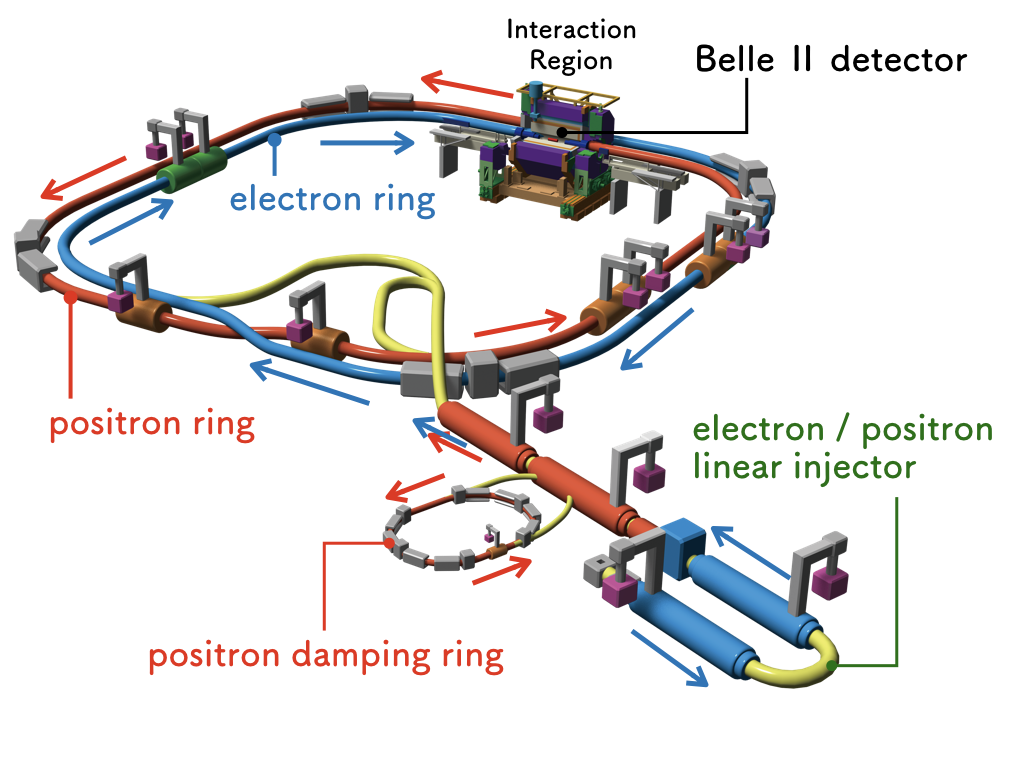
\includegraphics[width=0.8\columnwidth]{Figures/C02_SuperKEKB_and_BelleII/SperKEKB.png}
    \caption{Total recorded integrated luminosity up to now (weekly) \cite{Integrated_luminosity}. }
    \label{fig:integrated luminosity}
\end{figure}

\begin{figure}[htbp]
    \centering
    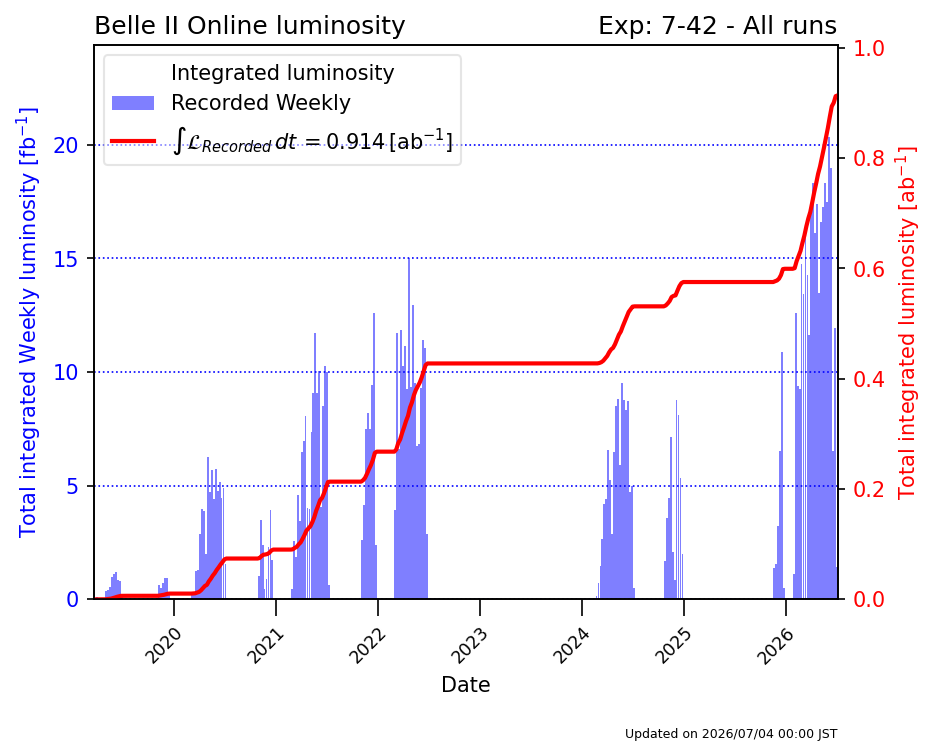
\includegraphics[width=0.8\columnwidth]{Figures/C02_SuperKEKB_and_BelleII/integrated_luminosity.png}
    \caption{Schematic drawing of SuperKEKB/BelleII facility \cite{Schematic_drawing_of_SuperKEKB/BelleII_facility}. }
    \label{fig:Schematic_drawing_of_SuperKEKB/BelleII_facility}
\end{figure}


\subsection{Collimator}
Collimator has important role to protect Belle II detector from back ground by blocking particles that deviated from its ideal trajectory. 


\begin{figure}[htbp]
    \centering
    \begin{minipage}{0.48\columnwidth}
        \centering
        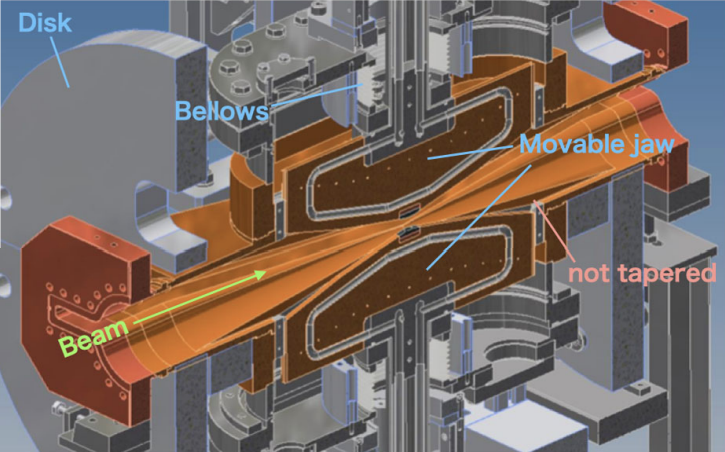
\includegraphics[width=\textwidth]{Figures/C02_SuperKEKB_and_BelleII/collimator_h.png}
    \end{minipage}
    \hfill
    \begin{minipage}{0.48\columnwidth}
        \centering
        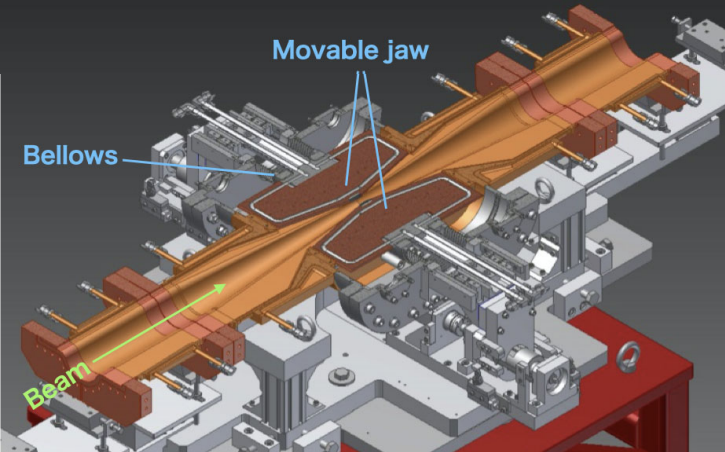
\includegraphics[width=\textwidth]{Figures/C02_SuperKEKB_and_BelleII/collimator_v.png}
    \end{minipage}
    \caption{Structure of horizontal (left) and vertical (right) collimator \cite{Ishibashi:2020rgt}.}
    \label{fig:structure of collimator}
\end{figure}


\subsection{Nano-beam scheme}
Instantaneous luminosity is written as bellows: 
\begin{align}
L
&= \frac{N_- N_+ n_b f_0}
{4\pi \sigma_x^* \sigma_y^*}
\qquad \text{(normal)}
\\
&= \frac{N_- N_+ n_b f_0}
{4\pi \sigma_{x,\mathrm{eff}}^* \sqrt{\varepsilon_y \beta_y^*}}
\qquad \text{(nano beam scheme)}
\\
&\simeq
\frac{\gamma_\pm}{2 e r_e}
\left(
\frac{I_\pm \xi_y^\pm}{\beta_y^{*\pm}}
\right)
\end{align}

where N is the number of particles in one bunch, $n_b$ is the number of bunch, $f_0$ is the revolutional frequency, $r_e$ is the classical radias of electron, $\beta_{y}^*$ is the vertical betatron function at the interaction point, I is the beam current, $\xi_y$ is the vertical beam-beam tune shift, $\gamma$ is the Lorentz factor. + means positron beam and - means electron beam. From this expression, $\beta_y^*$ should be small, I and $\xi$ should be large to improve luminosity. However, if we squeeze $\beta_y^*$ as small as the length of bunch( $\sigma_z$), luminosity can't be improved due to the hour-glass effect and synchro-betatron resonance. The hour-glass effect is that squeezing beam too much makes the bunch size large at the front end and the rear end, then the density becomes lower and causing stronger interaction with opposite beam. 

Nano-beam scheme scheme resolves this issue by colliding beams with large crossing angle in horizontal direction. 



\begin{figure}[htbp]
    \centering
    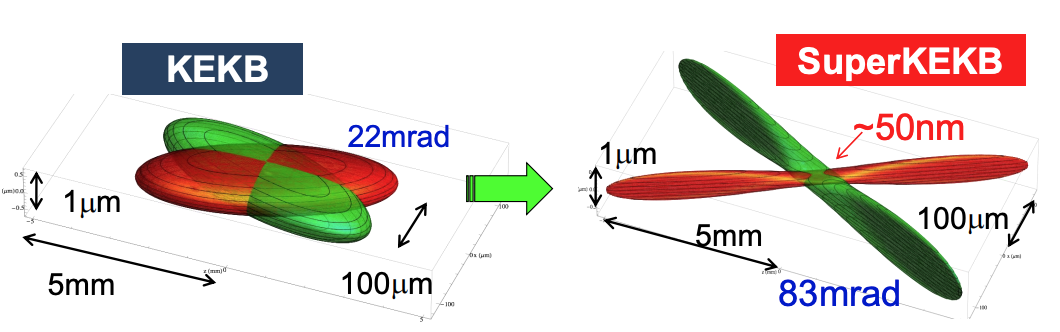
\includegraphics[width=1.0\columnwidth]{Figures/C02_SuperKEKB_and_BelleII/nanobeam_scheme.png}
    \caption{Nano beam scheme \cite{Nano_beam_scheme} }
    \label{fig:Nano beam cheme}
\end{figure}





\section{BelleII detector}
BelleII detector \cite{BelleII_detector}is a general purpose detector consisting of 7 sub-detectors, located at the interaction point of SuperKEKB. 

\subsection{Vertex detector}
PXD, pixcel detector is located at the most inner layer to measure vertex of decay particles. 

SVD, silicon vertex detector, has x layer strip silicon structure. 

CDC, central drift chamber, is the gas chamber with a diameter of 3m. 


\subsection{Particle identification}


\begin{figure}[htbp]
    \centering
    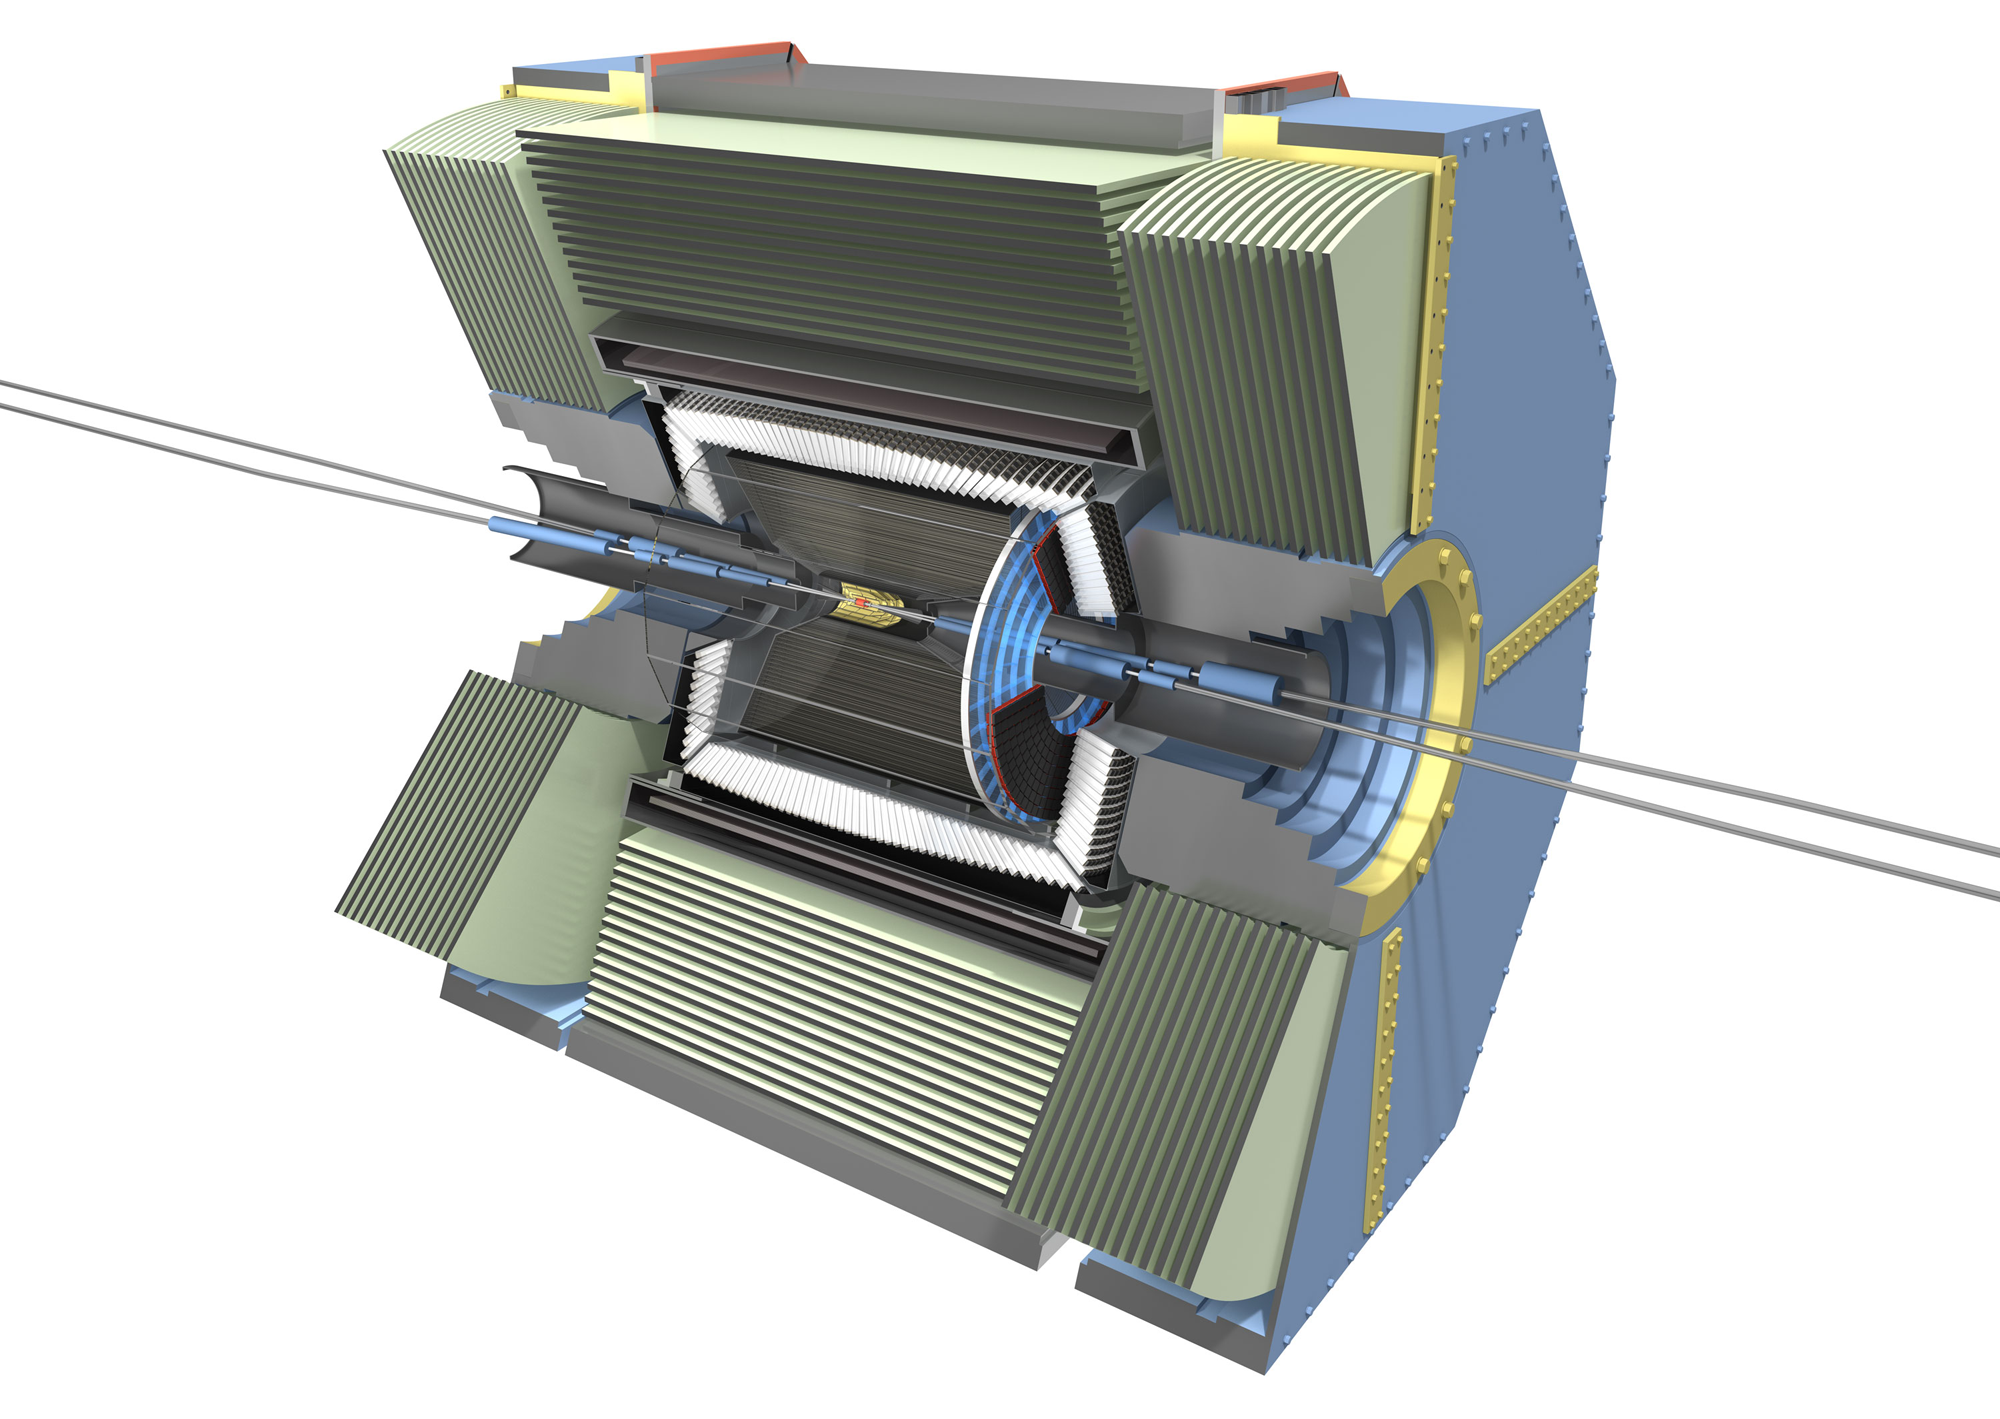
\includegraphics[width=0.8\columnwidth]{Figures/C02_SuperKEKB_and_BelleII/BelleII_detector.png}
    \caption{BelleII detector \cite{BelleII_detector}. }
    \label{fig:BelleII detector}
\end{figure}






Belle II Technical Design Report \cite{Belle-II:2010dht}

